\documentclass[output=paper,colorlinks,citecolor=brown
% ,hidelinks
% showindex
]{langscibook}

\author{Dafydd Gibbon\orcid{0000-0002-9825-5516}\affiliation{Bielefeld University}}

\title{Cohesive rhythms: choral narrative in Ega}

\abstract{This contribution combines functional, structural and acoustic explanations of a domain 'beyond words': how speech rhythm provides narrative cohesion and group bonding by caller entrainment with a choir during an orature event, recorded during fieldwork, in Ega, an endangered language isolate in south central Ivory Coast. The event in question is an oral narrative, a parable related in an interactive scenario by the village orator in two roles: as narrator, with feedback from his designated responder, and as caller in chanted interaction with the audience. First, a qualitative characterisation of coupling functions of speech rhythms is given, continued with a cyclical dynamic interaction model with specific rhythmical properties. The qualitative analyses are followed by a phonetic analysis based on annotation mining as a bridge leading to the quantitative signal processing of rhythm formants, and back to a qualitative interpretation of frequency properties of spectral peaks as resonant rhythm formants. While previous approaches have either selected functional or structural or acoustic analyses and representations of rhythm, the present study shows how these three approaches, taken together, can cohere and explain how speech rhythm patterns can be both physically grounded and functionally interpreted in context.}

%%%%%%%%%%%%%%%%%%%%%%%%%%%%%%%%%%%%%%%%%%%%%%%%%%%%
%%%%%%%%%%%%%%%%%%%%%%%%%%%%%%%%%%%%%%%%%%%%%%%%%%%%


\IfFileExists{../localcommands.tex}{
   \addbibresource{../localbibliography.bib}
   \newcommand{\orcid}[1]{}

\usepackage{orcidlink}

\usepackage{tabularx,multicol}
\usepackage{url}
\urlstyle{same}


\usepackage{langsci-optional}
\usepackage{langsci-lgr}
\usepackage{langsci-gb4e}

% for texlive 2022
\usepackage{langsci-branding} 

% Müller


% \usepackage{biblatex-series-number-checks}

% \usepackage{eng-date}

% \usepackage{german}%% Das Buch ist nicht deutsch. Hör auf, solche Sachen zu laden


% \usepackage{tikz-dependency}
% \usepackage{tikz}
% \usepackage{tikz-qtree}

% \usepackage{hologo}

% 3_pullum.tex

% This does not work complains about recommanding epsilon
% We use a special adapted version, which is in the repro.
\usepackage{langsci-textipa}



% 8_levine

\usepackage{./styles/lg-macro2}
\usepackage{bm}
\usepackage{umoline}
\usepackage{pifont}
\usepackage{pstricks,pst-node,pst-tree}
\usepackage{ulem}
\usepackage{mathrsfs}
\usepackage{bussproofs}




%\usepackage{tikz,tikz-qtree}

%\usepackage{gb4e0}
%\noautomath

%\usepackage[letterpaper,margin=1.2in]{geometry}



% 14_kornai

%\usepackage{xypic} % seems not to be needed
% \usepackage[matrix,arrow]{xy}
%\usepackage{amsmath}
% \usepackage{subcaption}
% \usepackage{wrapfig}


   
\SetupAffiliations{output in groups = false,
                   orcid placement = after,
                   separator between two = {\bigskip\\},
                   separator between multiple = {\bigskip\\},
                   separator between final two = {\bigskip\\}
                   }

% ORCIDs in langsci-affiliations 
\definecolor{orcidlogocol}{cmyk}{0,0,0,1}
\RenewDocumentCommand{\LinkToORCIDinAffiliations}{ +m }
  {%
    \,\orcidlink{#1}%
  }


\makeatletter
\let\thetitle\@title
\let\theauthor\@author
\makeatother

\newcommand{\togglepaper}[1][0]{
   \bibliography{../localbibliography}
   \papernote{\scriptsize\normalfont
     \theauthor.
     \titleTemp.
     To appear in:
     E. Di Tor \& Herr Rausgeberin (ed.).
     Booktitle in localcommands.tex.
     Berlin: Language Science Press. [preliminary page numbering]
   }
   \pagenumbering{roman}
   \setcounter{chapter}{#1}
   \addtocounter{chapter}{-1}
}

\newbool{bookcompile}
\booltrue{bookcompile}
\newcommand{\bookorchapter}[2]{\ifbool{bookcompile}{#1}{#2}}


% Cite and cross-reference other chapters
\newcommand{\crossrefchaptert}[2][]{\citet*[#1]{chapters/#2}, Chapter~\ref{chap-#2} of this volume} 
\newcommand{\crossrefchapterp}[2][]{(\citealp*[#1]{chapters/#2}, Chapter~\ref{chap-#2} of this volume)}
\newcommand{\crossrefchapteralt}[2][]{\citealt*[#1]{chapters/#2}, Chapter~\ref{chap-#2} of this volume}
\newcommand{\crossrefchapteralp}[2][]{\citealp*[#1]{chapters/#2}, Chapter~\ref{chap-#2} of this volume}

\newcommand{\crossrefcitet}[2][]{\citet*[#1]{chapters/#2}} 
\newcommand{\crossrefcitep}[2][]{\citep*[#1]{chapters/#2}}
\newcommand{\crossrefcitealt}[2][]{\citealt*[#1]{chapters/#2}}
\newcommand{\crossrefcitealp}[2][]{\citealp*[#1]{chapters/#2}}


\newcommand{\sub}[1]{\textsubscript{\scriptsize\textrm{#1}}}

% Müller

\newcommand{\page}{}

\let\citew\citet

\def\underRevision{Revise and resubmit}

\let\textbfemph\emph

\newcommand{\todostefan}[1]{\todo[color=orange!80]{\footnotesize #1}\xspace}
\newcommand{\todosatz}[1]{\todo[color=red!40]{\footnotesize #1}\xspace}

\newcommand{\inlinetodostefan}[1]{\todo[color=green!40,inline]{\footnotesize #1}\xspace}

\newcommand{\inlinetodoopt}[1]{\todo[color=green!40,inline]{\footnotesize #1}\xspace}
\newcommand{\inlinetodoobl}[1]{\todo[color=red!40,inline]{\footnotesize #1}\xspace}

\newcommand{\itd}[1]{\inlinetodoobl{#1}}
\newcommand{\itdobl}[1]{\inlinetodoobl{#1}}
\newcommand{\itdopt}[1]{\inlinetodoopt{#1}}

\newcommand{\addpages}{\todostefan{add pages}}

%% % taken from https://tex.stackexchange.com/a/95079/18561
\newbox\usefulbox

\makeatletter
\def\getslant #1{\strip@pt\fontdimen1 #1}

\def\skoverline #1{\mathchoice
 {{\setbox\usefulbox=\hbox{$\m@th\displaystyle #1$}%
    \dimen@ \getslant\the\textfont\symletters \ht\usefulbox
    \divide\dimen@ \tw@ 
    \kern\dimen@ 
    \overline{\kern-\dimen@ \box\usefulbox\kern\dimen@ }\kern-\dimen@ }}
 {{\setbox\usefulbox=\hbox{$\m@th\textstyle #1$}%
    \dimen@ \getslant\the\textfont\symletters \ht\usefulbox
    \divide\dimen@ \tw@ 
    \kern\dimen@ 
    \overline{\kern-\dimen@ \box\usefulbox\kern\dimen@ }\kern-\dimen@ }}
 {{\setbox\usefulbox=\hbox{$\m@th\scriptstyle #1$}%
    \dimen@ \getslant\the\scriptfont\symletters \ht\usefulbox
    \divide\dimen@ \tw@ 
    \kern\dimen@ 
    \overline{\kern-\dimen@ \box\usefulbox\kern\dimen@ }\kern-\dimen@ }}
 {{\setbox\usefulbox=\hbox{$\m@th\scriptscriptstyle #1$}%
    \dimen@ \getslant\the\scriptscriptfont\symletters \ht\usefulbox
    \divide\dimen@ \tw@ 
    \kern\dimen@ 
    \overline{\kern-\dimen@ \box\usefulbox\kern\dimen@ }\kern-\dimen@ }}%
 {}}
\makeatother

% 1_intro.tex

% For the block quote:

\usepackage[most]{tcolorbox}
\definecolor{linequote}{RGB}{224,215,188}
\definecolor{backquote}{RGB}{249,245,233}
\newtcolorbox{myquote}[1][]{%
    enhanced, breakable, 
    size=minimal,
    frame hidden, boxrule=0pt,
    sharp corners,
    colback=backquote,
    #1
}

% 2_gibson.tex


% Example(s) Environments
% 12pt, No new-lines after example number is printed

\newcounter{examplectr}
\newcounter{fnexamplectr}

% Note: don't use subexamples in footnotes.

% This line is to overcome a bug in cmu-art style: it prints counter
% values to the aux file using \theaux... rather than using \the...
\def\theauxexamplectr{\theexamplectr}

\newcounter{subexamplectr}
\def\theauxsubexamplectr{\thesubexamplectr}
\def\theauxfnexamplectr{\thefnexamplectr}

\renewcommand{\theexamplectr}{\arabic{examplectr}}
% This command causes example numbers to appear without following periods

\renewcommand{\thefnexamplectr}{\roman{fnexamplectr}}
% This command causes example numbers to appear without following periods

\renewcommand{\thesubexamplectr}{\theexamplectr\alph{subexamplectr}}
% This command gives the number of an example and subexample as e.g. 1a, 2b

\newlength{\wdth}
\newcommand{\strike}[1]{\settowidth{\wdth}{#1}\rlap{\rule[.5ex]{\wdth}{1pt}}#1}

\newcommand{\exref}[1]{(\ref{#1})}
% This command puts reference numbers with parentheses
% surrounding them 

% The environment ``examples'' gives a list of examples, one on each line,
% numbered with a lower case alphabetic character
\newenvironment{examples}%
   { \vspace{-\baselineskip}
     \begin{list}%
     \textrm{\alph{subexamplectr}.}%
     {\usecounter{subexamplectr}
     \setlength{\topsep}{-\parskip}
     \setlength{\itemsep}{-2pt}
     \setlength{\leftmargin}{0.5in}
     \setlength{\rightmargin}{0in} } }%
   { \end{list}}

% The environment ``myexample'' outputs an arabic counter ``examplectr''
% surrounded by parentheses.
\newenvironment{myexample}
   { \vspace{20pt}
     \noindent
     \begin{minipage}{\textwidth}    % minipage environment disallows
                 % breaks across pages

     \refstepcounter{examplectr}     % step the counter and cause this
                 % section to be referenced by the
                 % counter ``examplectr''
     (\arabic{examplectr})}%
   { \vspace{20pt}
     \end{minipage}}

\newenvironment{myfnexample}
   { \vspace{2pt}
     \noindent
     \begin{minipage}{\textwidth}    % minipage environment disallows
                 % breaks across pages

     \refstepcounter{fnexamplectr}     % step the counter and cause this
                 % section to be referenced by the
                 % counter ``examplectr''
     (\roman{fnexamplectr})}%
   { \vspace{2pt}c
     \end{minipage}}
    
\newcommand*\circled[1]{\tikz[baseline=(char.base)]{
            \node[shape=circle,draw,inner sep=2pt] (char) {#1};}}



% 3_pullum.tex


% %%%  GKP:  I put in these pointless commands to kill off a bug elsewhere
% %%%        that tries to \newcommand \it (etc.) as \itshape (etc.), but
% %%%        fails because they haven't been defined.
% \newcommand{\it}{\relax}
% \newcommand{\bf}{\relax}
% \newcommand{\sc}{\relax}
% \newcommand{\rm}{\relax}

%%% GKP:  Two additional commands that I need
\newcommand{\data}[1]{\textit{#1}}
\newcommand{\blank}{\rule{1.2em}{0.5pt}}



% 8_levine

% ???
%\renewcommand{\emph}{\textit}
%\renewcommand{\em}{\it}

% not used \newcommand{\cites}[1]{\citeauthor{#1}'s~\citeyearpar{#1}}

% \renewcommand{\SetInfLen}{\setpremisesend{0pt}\setpremisesspace{10pt}\setnamespace{0pt}}

\newcommand{\pt}[1]{\ensuremath{\mathsf{#1}}}
\newcommand{\ptv}[1]{\ensuremath{\textsf{\textsl{#1}}}}

%\newcommand{\sv}[1]{\ensuremath{\bm{\mathcal{#1}}}}
\newcommand{\sv}[1]{\ensuremath{\mathcal{#1}}}

\newcommand{\sX}{\sv{X}}
\newcommand{\sF}{\sv{F}}
\newcommand{\sG}{\sv{G}}
%
% \renewcommand{\lex}{\SF}
% \renewcommand{\syncat}[1]{\ensuremath{\mathrm{#1}}}
% \newcommand{\syncatVar}[1]{\ensuremath{\mathit{#1}}}
%
% \newcommand{\RuleName}[1]{\textrm{#1}}
%
% \newcommand{\SemTyp}{\textsf{Sem}}
%
% \newcommand{\something}{\vdots\,\,\,\,\,\,\vdots}
%
% \newcommand{\pb}{\phantom{[}}
%
% \renewcommand{\E}{\ensuremath{\bm{\epsilon}}\xspace}
%
% \newcommand{\greeka}{\upalpha}
% \newcommand{\greekb}{\upbeta}
% \newcommand{\greekd}{\updelta}
\newcommand{\greekp}{\upvarphi}
\newcommand{\greekr}{\uprho}
\newcommand{\greeks}{\upsigma}
% \newcommand{\greekt}{\uptau}
% \newcommand{\greeko}{\upomega}
% \newcommand{\greekz}{\upzeta}
%
% % Do not do this!!!!!
% % \renewcommand{\labelenumi}{(\roman{enumi})}
%
% \newcommand{\upa}[2]{\ensuremath{\syncat{#1}|\syncat{#2}}}
% \newcommand{\dna}[2]{\upa{#2}{#1}}
%

%
% \newcommand{\Lemma}{\ensuremath{\vdots\hskip.5cm\vdots}\noLine}
%
% \newcommand{\la}{\ensuremath{\langle}}
% \newcommand{\ra}{\ensuremath{\rangle}}
%
% \renewcommand{\I}{\iota}
%
% \renewcommand{\sem}{\ensuremath}
%
% \newcommand{\LemmaShort}{\ensuremath{\vdots\hskip.2cm\vdots\hskip.2cm\vdots}\noLine}
% \newcommand{\LemmaShortAlt}{\ensuremath{\vdots\hskip.2cm\vdots}}
%
%
% \newcommand{\NoSem}{%
% \renewcommand{\LexEnt}[3]{##1; \syncat{##3}}
% \renewcommand{\LexEntTwoLine}[3]{\renewcommand{\arraystretch}{.8}%
% \begin{array}[b]{l} ##1;  \\ \syncat{##3} \end{array}}
% \renewcommand{\LexEntThreeLine}[3]{\renewcommand{\arraystretch}{.8}%
% \begin{array}[b]{l} ##1; \\ \syncat{##3} \end{array}}}
%
%
% \newcommand{\NoSemVar}{%
% \renewcommand{\LexEnt}[3]{##1; \syncat{##3}}
% \renewcommand{\LexEntTwoLine}[3]{\renewcommand{\arraystretch}{.8}%
% \begin{array}{l} ##1;  \\ \syncat{##3} \end{array}}
% \renewcommand{\LexEntThreeLine}[3]{\renewcommand{\arraystretch}{.8}%
% \begin{array}{l} ##1; \\ \syncat{##3} \end{array}}}
%
% \newcommand{\vs}{\raisebox{.05em}{\ensuremath{\upharpoonright}}}
%
% \newcommand{\AXX}[1]{\raisebox{-7mm}{\ensuremath{#1}}}
%
% \newcommand{\hypml}[2]{\left[\!\!#1\!\!\right]^{#2}}
%
% \newcommand{\alt}[2]{$\left\{\begin{array}{c}
% \hskip-.7ex\textrm{#1}\hskip-.7ex \\
% \hskip-.7ex\textrm{#2}\hskip-.7ex
%         \end{array}
% \right\}$}
%
% \newcommand{\altalt}[2]{\{#1/#2\}}
%
%
%
% \newcommand{\altt}[3]{$\left\{\begin{array}{c}
% \hskip-.7ex\textrm{#1}\hskip-.7ex \\
% \hskip-.7ex\textrm{#2}\hskip-.7ex \\
% \hskip-.7ex\textrm{#3}\hskip-.7ex
% \end{array}
% \right\}$}
%
% \newcommand{\alttt}[4]{$\left\{\begin{array}{c}
% \hskip-.7ex\textrm{#1}\hskip-.7ex \\
% \hskip-.7ex\textrm{#2}\hskip-.7ex \\
% \hskip-.7ex\textrm{#3}\hskip-.7ex \\
% \hskip-.7ex\textrm{#4}\hskip-.7ex
% \end{array}
% \right\}$}
%
%
% %%%%for bussproof
%
% \def\defaultHypSeparation{\hskip0.1in}
% \def\ScoreOverhang{0pt}
%
%
% %%\newcommand{\MultiLine}[1]{\renewcommand{\arraystretch}{.8}%
% %%\ensuremath{\begin{array}{l} #1 \end{array}}}
%
\newcommand{\MultiLine}[1]{\renewcommand{\arraystretch}{.8}%
\ensuremath{\begin{array}[b]{l} #1 \end{array}}}

%
%
% \newcommand{\MultiLineMod}[1]{%
% \ensuremath{\begin{array}[t]{l} #1 \end{array}}}
%
%
% %%%%%\AFourMargin
% %%\JLSubmissionMargin
%
% %%\setlength\topmargin{-1cm}
% %%\setlength\textheight{23cm}
% %%%%%\setlength\textwidth{13.5cm}
%
% %\setstretch{1.2}
%
% % not used \newcommand{\hyp}[2]{[ #]^{#2}}
%
\newcommand{\LexEnt}[3]{#1; \ensuremath{#2}; \syncat{#3}}
%
% \newcommand{\LexEntTwoLine}[3]{\renewcommand{\arraystretch}{.8}%
% \begin{array}[b]{l} #1; \\ \ensuremath{#2};  \syncat{#3} \end{array}}
%
% \newcommand{\LexEntThreeLine}[3]{\renewcommand{\arraystretch}{.8}%
% \begin{array}[b]{l} #1; \\ \ensuremath{#2}; \\ \syncat{#3} \end{array}}
%
%
% \newcommand{\LexEntFiveLine}[5]{\renewcommand{\arraystretch}{.8}%
% \begin{array}{l} #1 \\ #2; \\ \ensuremath{#3} \\ \ensuremath{#4}; \\ \syncat{#5} \end{array}}
%
%
% \newcommand{\LexEntFourLine}[4]{\renewcommand{\arraystretch}{.8}%
% \begin{array}{l} \pt{#1} \\ \pt{#2}; \\ \syncat{#4} \end{array}}
%
% \newcommand{\ManySomething}{\renewcommand{\arraystretch}{.8}%
% \raisebox{-3mm}{\begin{array}[b]{c} \vdots \,\,\,\,\,\, \vdots \\
% \vdots \,\,\,\,\,\, \vdots \end{array}}}
%
%
% \newcommand{\lemma}[1]{\renewcommand{\arraystretch}{.8}%
% \begin{array}[b]{c} \vdots \,\,\,\,\,\, \vdots \\ #1 \end{array}}
%
% \newcommand{\lemmarev}[1]{\renewcommand{\arraystretch}{.8}%
% \begin{array}[b]{c} #1 \\ \vdots \,\,\,\,\,\, \vdots \end{array}}
%
% \newcommand{\p}{\ensuremath{\upvarphi}}
%
% \newcommand{\Not}{\leavevmode\llap{\textbf{\smc{NOT:}} }}
%
% \newcommand{\Conj}{\fs{\bsp{\mathit{X}}{\mathit{X}}}{\mathit{X}}}
% \newcommand{\ConjY}{\fs{\bsp{\mathit{Y}}{\mathit{Y}}}{\mathit{Y}}}
% \newcommand{\sameLE}{\dna{(\upa{(\upa{S}{\mathit{X}})}{NP})}{(\upa{S}{\mathit{X}})}}
%
% \newcommand{\derivcenter}[2][1.1]{%
% \SetInfLen
% \attop{\vskip3ex
% \resizebox{#1\linewidth}{!}{\hskip-#1in
% #2}}}
%
% \newcommand{\derivcenterAlt}[2][.98]{%
% \SetInfLen
% \attop{\vskip3ex
% \resizebox{#1\linewidth}{!}{\hskip-#1in \hskip.5in
% #2}}\vspace{.5ex}}
%
% \renewcommand{\O}{\circ}  Do not recommand!
\newcommand{\BobsO}{\circ}
%
% \newcommand{\derivcenterMod}[2][1.1]{%
% \renewcommand{\LexEntThreeLine}[3]{\renewcommand{\arraystretch}{.8}%
% \raisebox{.4ex}{\ensuremath{\begin{array}{l} ##1; \\ \ensuremath{##2}; \\ \syncat{##3} \end{array}}}}
% \SetInfLen
% \attop{\vskip3ex
% \resizebox{#1\linewidth}{!}{\hskip-#1in
% #2}}}
%
%
% \newcommand{\shortarrow}{\xspace\hskip-1.2ex\scalebox{.5}[1]{\ensuremath{\bm{\rightarrow}}}\hskip-.5ex\xspace}
%
% \newcommand{\SemInt}[1]{\mbox{$[\![ \textrm{#1} ]\!]$}}
%
% \def\maru#1{{\ooalign{\hfil
%   \ifnum#1>999 \resizebox{.25\width}{\height}{#1}\else%
%   \ifnum#1>99 \resizebox{.33\width}{\height}{#1}\else%
%   \ifnum#1>9 \resizebox{.5\width}{\height}{#1}\else #1%
%   \fi\fi\fi%
% \/\hfil\crcr%
% \raise.167ex\hbox{\mathhexbox20D}}}}
%
\newcommand{\HypSpace}{\hskip-.8ex}
\newcommand{\RaiseHeight}{\raisebox{2.2ex}}
% \newcommand{\RaiseHeightLess}{\raisebox{1ex}}
%
% \newcommand{\fW}{\ensuremath{\mathfrak{W}}}
%
\newcommand{\ThreeColHyp}[1]{\RaiseHeight{\Bigg[}\HypSpace#1\HypSpace\RaiseHeight{\Bigg]}}
% \newcommand{\TwoColHyp}[1]{\RaiseHeightLess{\Big[}\HypSpace#1\HypSpace\RaiseHeightLess{\Big]}}
%
%
% %\newcommand{\maskref}[1]{\textsl{\textbf{[reference omitted for refereeing]}}}
% \newcommand{\maskref}[1]{#1}
%
% \newcommand{\DerivSize}{\small}
% \newcommand{\AppDerivSize}{\footnotesize}
%
% \renewcommand{\sem}{\ensuremath}


% \newcommand{\greekp}{{\color{green}π}}
% \newcommand{\greekr}{{\color{green}\textrho}}
% \newcommand{\greeks}{{\color{green}\textsigma}}
\newcommand{\ptfont}[1]{\texttt{#1}}                % what does ptfont do? Where is it defined?
                                % Question
%\newcommand{\ptfont}{\ttfamily}

%\newcommand{\grey}{\color{gray}}
\newcommand{\grey}[1]{\colorbox{mycolor}{#1}}
\definecolor{mycolor}{gray}{0.8}

\newcommand{\gap}{\longrule}
\newcommand{\gp}{\gap}
\newcommand{\vs}{\raisebox{.05em}{\ensuremath{\upharpoonright}}}
% \newcommand{\sub}[1]{\textsubscript[#1]}
\newcommand{\E}{\emph}
\newcommand{\B}{\textbf}
\newcommand{\f}{{\color{green}f}}  % Question what does f do? It does not have any output in the
                                % original PDF
%\newcommand{\Lemma}{{\color{pink}Lemma}}
\newcommand{\Lemma}{\ensuremath{\vdots\hskip.5cm\vdots}\noLine}

%\newcommand{\calP}{{\color{pink}calP}} % Sebastian
\newcommand{\calP}{\ensuremath{\mathcal{P}}}


\newcommand{\maru}[1]{\ooalign{\hfil#1\/\hfil\crcr
      \raise.05ex\hbox{\LARGE\mathhexbox20D}}}


%\newcommand{\sem}[2][M\!,g]{\mbox{$[\![ \mathrm{#2} ]\!]^{#1}$}}
\newcommand{\sem}{\ensuremath}

%
\newcommand{\trns}[1]{\textbf{#1}\xspace}

\newcommand{\bs}{{\textbackslash}}
\newcommand{\bsl}{{\bs}}


\newcommand{\fb}[1]{\textsubscript{#1}}

\newcommand{\syncat}[1]{\ensuremath{\mathrm{#1}}}
\newcommand{\term}[1]{\textit{#1}}
\newcommand{\LemmaAlt}{\ensuremath{\vdots\hskip.5cm\vdots}}

%\renewcommand{\O}{ø}

   %% hyphenation points for line breaks
%% Normally, automatic hyphenation in LaTeX is very good
%% If a word is mis-hyphenated, add it to this file
%%
%% add information to TeX file before \begin{document} with:
%% %% hyphenation points for line breaks
%% Normally, automatic hyphenation in LaTeX is very good
%% If a word is mis-hyphenated, add it to this file
%%
%% add information to TeX file before \begin{document} with:
%% %% hyphenation points for line breaks
%% Normally, automatic hyphenation in LaTeX is very good
%% If a word is mis-hyphenated, add it to this file
%%
%% add information to TeX file before \begin{document} with:
%% \include{localhyphenation}
\hyphenation{
    par-a-digm
}

\hyphenation{
    par-a-digm
}

\hyphenation{
    par-a-digm
}

   \boolfalse{bookcompile}
   \togglepaper[23]%%chapternumber
}{}

\graphicspath{ {./figures/} }

\begin{document}
\maketitle

%%%%%%%%%%%%%%%%%%%%%%%%%%%%%%%%%%%%%%%%%%%%%%%%%%%%
%%%%%%%%%%%%%%%%%%%%%%%%%%%%%%%%%%%%%%%%%%%%%%%%%%%%

\section{Speech rhythms in village orature}

The present case study in the documentation and description of Ega, a language isolate of south-central Ivory Coast, is about the physical properties, structure and meaning of rhythms in interactive discourse. The study explores a communal orature event in Ega and its underpinnings in the rhetorical and poetic rhythms of speech. The genre of the event is a parable told through interaction among \textit{narrator-responder} and \textit{caller-choir} participants, where the audience is the \textit{choir}, and with variability of mutual rhythm entrainment in different phases of the narrative. The study relates closely to the emphasis in \cite{sakeleverett2012} on contributions of multidisciplinary methods to fieldwork, dialogue description and documentation of language and culture.

The data consist of the sound track of the video recording of the parable, which is narrated by an accomplished orator, the \textit{chef du village}, to his fellow villagers in the Ega-speaking region of Ivory Coast \cite{rossinigibbon2011}. The general framework for the case study is description and documentation of an endangered language \cite{gibbonbowbirdhughes2004}, with the aim of understanding some of the discourse skills of the community by combining brief functional and structural accounts as background for a contemporary prosodic phonetic analysis, in search of both hermeneutic interpretation and causal physical grounding for speech rhythms.

\begin{figure}[ht]
\centering
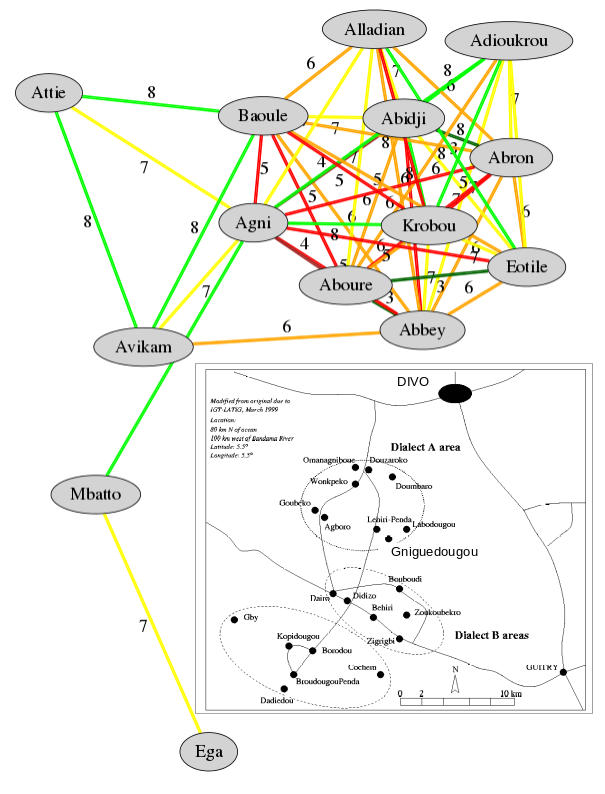
\includegraphics[width=0.65\textwidth]{gibbon_figure01.png}
\vspace{-10pt}
\caption{\label{fig:fig01}Unsupervised clustering of Ivory Coast Kwa languages derived from phoneme feature vectors (source: Atlas Linguistique des Langues Kwa, \cite{herault1983}). Colours and line lengths represent Hamming distances between phoneme inventory vectors. Insert: Sketch map of the Ega enclave in south-central Ivory Coast.}
\end{figure}

\begin{figure}[ht]
\centering
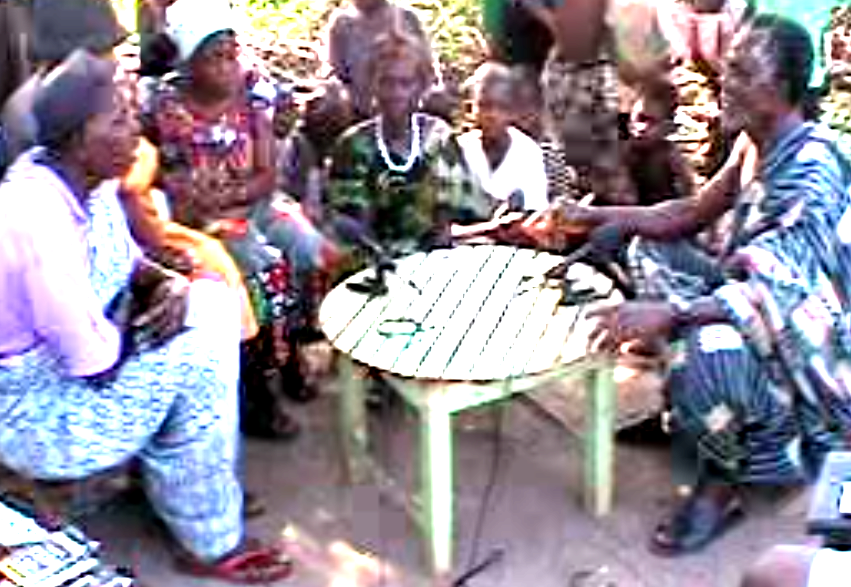
\includegraphics[width=0.65\textwidth]{gibbon_figure02.png}
\caption{\label{fig:fig02}Recording scenario with narrator (right), responder (left) and audience. (Video frame by permission of the participants.)}
\end{figure}

The video data were recorded on 6th March 2001, during fieldwork on the Ega language in Gnieguédougou village, Ivory Coast, an enterprise which was cut short by the Ivorian civil war. The data are consequently rare and sparse, and quantitative phonetic analysis has therefore to be subordinated to qualitative interpretation and structural modelling, and to a final qualitative interpretation of the quantitative results in terms of initial assumptions and predictions. The direction taken in this contribution has the character of a travelogue about discovering discourse rhythms, their functionality, their structure and their physical form.

The language Ega (ISO 639-3 \textit{ega}) is an endangered Niger-Congo tone language isolate in south central Ivory Coast. The endangerment of the language results from several factors, including the gradual failing of intergenerational transmission due to the dominance of French in schooling and influence from the enclaving Eastern Kru dialect related to Lakota Dida (ISO 639-3 \textit{dic}) as spoken in neighbouring Divo.

Ega has been tentatively assigned to the Kwa subgroup \cite{bolerichard1983, connellahouagibbon2002, salffner2004}. A sceptical view is taken in \cite{blench2015, blench2017} of the closeness of the language to other Ivory Coast Kwa languages or other neighbouring Niger-Congo subgroups. Ega community members in the social media see the Ega as autochthonous, surrounded by invading ethnic groups. Ega is regarded with some suspicion as a `secret language' by Dida speakers, whose name for the community and the language is Diès, a term resented by many Ega as a colonial invention. The outsider status of Ega in relation to other Ivory Coast Kwa languages is shown in \cite{gibbonweb2014}, using unsupervised clustering of pairwise phoneme inventory distances between Kwa languages,\footnote{$http://wwwhomes.uni-bielefeld.de/gibbon/DistGraph/distgraph-kwa.html$} based on legacy data from the \textit{Atlas des langues Kwa} \cite{herault1983}. The visualisation in Figure\,\ref{fig:fig01} shows the linguistic isolate status of Ega, which matches its geographical and social isolate status as an enclave in a Kru area.

The orature session takes place in a typical Niger-Congo village scenario involving an orator with two roles: as \textit{narrator} of the parable, with a designated backchannel \textit{responder}, and as the \textit{caller} who elicits \textit{choir} responses from the audience in interactive chanted segments of the session, cf. Figure\,\ref{fig:fig02}. The participant role relations can be summarised as follows:
\begin{quotation}
\centering
[\,[\,[\textit{narrator-caller}, \textit{responder}\,], \textit{audience-choir}\,], \textit{observer-fieldworker}\,]
\end{quotation}
The parable concerns a faithless young bride-to-be who left her promised bridegroom and is on her way to the next village to marry her new-found future husband. She is fruitlessly warned by a twittering bird with a prophecy about her impending end at the hands of her formerly betrothed suitor, who had worked for free for her father to win her hand. Alas, the girl did not understand. The bride and the suitor met along the way, he reproached and threatened her, she spat at him, whereupon the prophecy came true. The parable closes with the moral that one should learn other languages like the fieldworkers are doing, meant as a kind gesture by the orator. But the real linguistic punchline is more subtle: the birdsong, with \textit{caller} and \textit{choir} turns, is actually in Dida, the enclaving Eastern Kru language, not in endangered Ega.

The approach taken in the present study is to concentrate on this one orature session and explore the rhetorical and musical rhythms which characterise the interactive narration; for a more extensive treatment of similar orature, cf. \cite{gibbon4urua2022}. In the following section, a brief qualitative linguistic outline of the functions and forms of the narration is given, as a basis for interpreting phonetically analysed rhythms. Section 3 continues with a hybrid qualitative-quantitative analysis of the speech recording annotated with turn-taking roles and Section 4 provides a detailed spectral analysis of the session in the frequency domain, following the principles of Rhythm Formant Theory. In Section 5, conclusions are drawn about orature rhythm, its functions, structure and forms.

%%%%%%%%%%%%%%%%%%%%%%%%%%%%%%%%%%%%%%%%%%%%%%%%%%%%%%%%%%%%%%%%%%%%%%%%%%
%%%%%%%%%%%%%%%%%%%%%%%%%%%%%%%%%%%%%%%%%%%%%%%%%%%%%%%%%%%%%%%%%%%%%%%%%%

\section{The ubiquity of rhythms: function, form and sound}

Rhythms are a key topic in many disciplines, not only in the study of music and speech, but in fields from astronomy and oceanography through econometrics to medicine, with cardiology and neurology in the forefront \cite{lewalterluederitz2010, huangetal1998}. The algorithms used in the analysis of temporal regularities and irregularities in these fields are closely related to the low frequency (LF) spectral analysis approach of this contribution, and equally closely related to the algorithms of popular smartphone song-recognition applications \cite{wangshazam2003}. The concept of rhythm which underlies the present approach is also related to the account of expectations created by sequences of similar pitch accents in English \cite{dilley2005} and can be formulated as follows, with \textit{natural rhythms} understood in the traditional sense of temporally regular sequences of beats:

\begin{quotation}
\noindent A \textit{natural rhythm} is perceived, and can be measured, when a series of similarly structured events occurs with a specific frequency at approximately equal intervals in time and motivates a prediction of a further similarly structured event after a similar interval.\footnote{It may be helpful to note that the expectation created by a rhythm is conceptually related to the econometric concept of \textit{Granger Causality} in time series, though without necessarily implying a rhythm: ``A time series X is said to Granger-cause Y if it can be shown [...] that those X values provide statistically significant information about future values of Y.'' (Wikipedia; p.c. A.\,J.\,Gibbon)}
\end{quotation}

In speech, music and dance, however, rhythm has communicative functionality which goes beyond the physical patterns of natural rhythms and occasions \textit{synchronisation} or \textit{rhythmic entrainment} among the interlocutors \cite{cumminsport1998, indenmaliszwagnerwachsmuth2012, rathckeetaltapping2021}:

\begin{quotation}
\noindent A \textit{behavioural rhythm} fulfils the conditions for producing a \textit{natural rhythm} and furthermore entrains perceptual synchronisation in its hearers.
\end{quotation}

In phonetics the main paradigm which uses this methodology is \textit{speech modulation theory} \cite{ohala1992, traunmueller1994, toddbrown1994, odellnieminen1999, barbosa2002, galvesetal2002, tilsenjohnson2008, indenmaliszwagnerwachsmuth2012, tilsenarvaniti2013, gibbonjipa2021}, in which beat \textit{frequency}, \textit{magnitude} and \textit{bandwidth} are the main properties of rhythms, and rhythms are generated by coupled oscillators and decoded in the frequency domain by a variety of spectral analysis algorithms. The present study uses a further development of Modulation Theory, Rhythm Formant Theory (RFA) \cite{gibbonjipa2021}, in which rhythm-characterising low frequency (LF) spectral peaks between approximately 10\,Hz and 0.01\,Hz are interpreted functionally as LF rhythm formants, by analogy with the spectral peaks of high frequency (HF) phone formants. The relevant aspects of RFA are outlined in Section 3.

\subsection{Linguistic, rhetorical and poetic rhythms}

Phonological and phonetic descriptions of rhythm tend to be concerned with the very brief timing patterns of ``linguistic rhythm'', in the words of \cite{libermanprince1977}, of syllable, word and phrase sequences. In phonetic terms, the periods of such rhythms tend to be between about 100\,ms for shorter syllables and 1\,s to 3\,s for phrases and sentences, corresponding to beat rates or frequencies between about 10\,Hz and 0.3\,Hz.

However, as studies in interactional linguistics show \cite{couperkuhlenselting2017}, much longer prosodic domains are called for in registers such as conversation, story-telling (as with the Ega parable), or speeches. For example, the duration of the complete Ega orature event is 300\,s, and very long-term LF rhythms with rhetorical functionality span the entire event.

As a poetic feature, rhythm is a configurative indicator of cohesion, which can be present in different types and degrees with different functionalities throughout a poetic event \cite{wagner2010}. The poetic discourse of the selected parable calls for description in terms of the metalocutionary dimension of \textit{coupling} \cite{levin1962}: the iteration of functionally relevant sound features which create a layer of ritualised cohesion superimposed over the grammatical structure of locutions, by means of iterative \textit{alliteration}, \textit{assonance} and \textit{rhyme}, and by the iterative patterns of performed rhythms, conventional metres, stanzas, refrains or the strophe-strophe-bridge-strophe patterns of popular music. Of all the available coupling parameters, only rhythm, as a variable iterative cohesion indicator, which may or may not align closely with grammatical structures or conventional metres, is picked out for discussion in the present case study.

The multiple long-term rhythms of discourse are referred to in the present context as \textit{rhetorical rhythms} or \textit{discourse rhythms}. Their multilevel intonation counterparts are sometimes refererred to in the literature as ``minor tone groups'', ``major tone groups'' \cite{trim1959} and, in longer time intervals, as ``minor paratones'' and ``major paratones'' \cite{yuleparatone1980}. The `prosodic hierarchy', a key theme in phonology, is only addressed indirectly in this study; hierarchical structure figures not in terms of a hierarchy of strict constituent inclusion (cf. the stress hierarchy of \cite{chomskyhalle1968} and the prosodic hierarchy of \cite{selkirk1984}), which are closely associated with grammatical structures, but in terms of a spectral scale of periodicities of different frequencies which are measurable in the physical speech signal.

\subsection{Metalocutionary functions}

The central question in the present section, which requires some background discussion, concerns rhythms as a meaningful component of utterances. A related and more frequently discussed issue is the analogous question of speech melodies as meaningful components of utterances, though these are not discussed here. The starting point for capturing the meanings of rhythms is the traditional concept of parallel information channels in spoken language: the rhythms and melodies of prosody, and the sounds, syllables, words and phrases of locutions. The parallel channel approach has been shared by most traditional intonation and stress textbook models for more than a century (for overviews see \cite{gibbon1976, arvaniti2022}), by speech engineering approaches \cite{morikawafujisaki1976, thartcohen73, dutoit2001, fujisaki2004} and, in phonology, with the exception of \cite{chomskyhalle1968}, by the popular metrical and autosegmental models \cite{barnesshattuckhufnagel2022}.

The core meanings of locutions are propositional \cite{Austin1962}, while the core meanings of prosodic forms are metalocutionary \cite{gibbon1976, gibbonmetalocution1981} and refer indexically to semantic features of the utterance and pragmatic features of the utterer:
\begin{itemize}
\item \textit{Semantic metadeixis} with respect to utterance locutions, in that rhythmic beats and beat sequences (such as pitch and duration accents, nuclear, contrastive and emphatic accents and sequences of these) \textit{denote} (or: \textit{refer to} or \textit{point at}) the real-time physical temporal locations of locutionary components which relate to information structure (as deictic gestures point in real-time and real space at components of the environment). Traditional terms for these metadeictic functions are \textit{culminative} for accents, \textit{configurative} for rhythmic and melodic groups, and \textit{delimitative} for boundary effects.
\item \textit{Pragmatic indexicality}, with respect to the utterer, with interpersonal indications of attitudes, emotions, beliefs, turn exchange control, as characteristics of the speaker such as sex, age, health, social status, physical and social proximity or distance \cite{gibbon1976, hirschbergpierrehumbert1986}.
\end{itemize}
Pragmatic indexical metalocutionary meanings are also conveyed in the locutionary channel itself by subjective adverbs, discourse particles and other lexical items with appraisive pragmatic features.

Lexical prosodic forms, such as phonemic and morphosyntactic tones and lexical pitch accents, have direct contrastive and syncategorematic functions and are tightly synchronised with head syllables of locutionary lexical items. In addition to some direct influence from segments, particularly consonants, tonal forms are partly independent of syllable components in the sense that they may undergo sandhi processes such as terracing and tonal assimilation without reference to locutionary properties \cite{gibbonfstone1987, jansche1998}. These lexical prosodic conditions also characterise the 3 phonemic and morphosyntactic level tones of the Ega language \cite{connellahouagibbon2002}.

Supralexical prosodic forms such as metadeictic pitch accents and intonation boundary and contour patterns are less tightly synchronised with the heads of the items they denote. Accentual and boundary features, also in tone languages such as Tem (Togo, ISO 639-3 \textit{kdh}) \cite{tchagbale2001}, Ega, and also Mandarin \cite{duanmu2007}, may include speech tempo deceleration with syllable lengthening, pitch upstep and downstep and increased pitch range, not only lexical tonal features such as relative pitch height, pitch range and pitch contour. In Ega narration, multimodal features of manual gesture, facial gesture and posture, as shown in Figure\,\ref{fig:fig02}, are part of the metalocutionary complex \cite{rossinigibbon2011}, but are not within the scope of the present contribution.

Speech rhythms in the Ega parable distinguish different kinds of prosodic cohesion in the narrative exchanges between the \textit{narrator} and his \textit{responder} on the one hand, and interactive choral exchanges between the \textit{caller} and the \textit{choir}, on the other hand, as the acoustic phonetic analyses in the following sections show. The rhythms of the narrative exchanges have the function of structuring cohesive propositional groups, while the rhythmic entrainment of the choral exchanges has an additional function of creating explicit backchannel agreement and social bonding among the participants along a functional scale between mutual entrainment to shared rhythmic patterns at the one end of the scale and relatively arhythmic patterns at the other end. The present data tend to show the former case, with cohesive rhythms associated with narration structure by an individual speaker, and with entrainment and bonding created by rhythms contributing to the aesthetic and social value of interactive choral chanting.

\subsection{Cyclic models for multiple rhythms}

The aim of the present section is to present a viable \textit{dynamic functional model} for the static participant model of [\,[\,[\textit{narrator-caller}, \textit{responder}\,], \textit{audience-choir}\,], \textit{observer-fieldworker}\,], in the sense that transitions between states in the dialogue are modelled, and map to long-term rhythms in the interlocution.

In structural terms, a rhythm is an iterative sequence of beats or waves which can be modelled by an iterative finite machine (finite state automaton, FSA), with multiple cycles, and which functions as a system of coupled oscillators \cite{cumminsport1998, odellnieminen1999, barbosa2002}. A little justification for using cyclical linear models is in order, since more powerful but less realistic models tend to be preferred in linguistics. However, many grammatical word and phrase structures are right-branching or left-branching, indicating that in computational formal grammar terms a fully centre-recursive Chomsky Type 2 (context-free, phrase structure) grammar is not necessary, and that a Type 3 (linear, regular) grammar is sufficient.

Type 3 recursion can be efficiently implemented as iteration with linear time and finite memory space process; this is not the case with general Type 2 languages. This has been clearly demonstrated in the `recursion debate' \cite{karlsson2010}. General recursion as a property of thought rather than language is proposed by \cite{everett2016}; other scholars (overview in \cite{gibbongriffiths2017}) suggest that communication with the more general recursion of thought was made possible partly by ritual rehearsal and (as in mathematics) by the invention of writing, which allows for extended processing time and permits the use of additional memory space in external media.

Another key difference is that for any Type 3 grammar there is an equivalent FSA (or FS transducer, FST, if tree output is also desired), with realistic processing properties of finite memory and linear time as a function of the size of the input. Cyclical FSAs are ubiquitous in many areas of computational linguistics, especially in morphology, phonology and prosody. It is assumed here, until the contrary is demonstrated, that FSAs and FSTs are the formal devices needed for the description of rhythms.
 
\begin{figure}[ht]
\centering
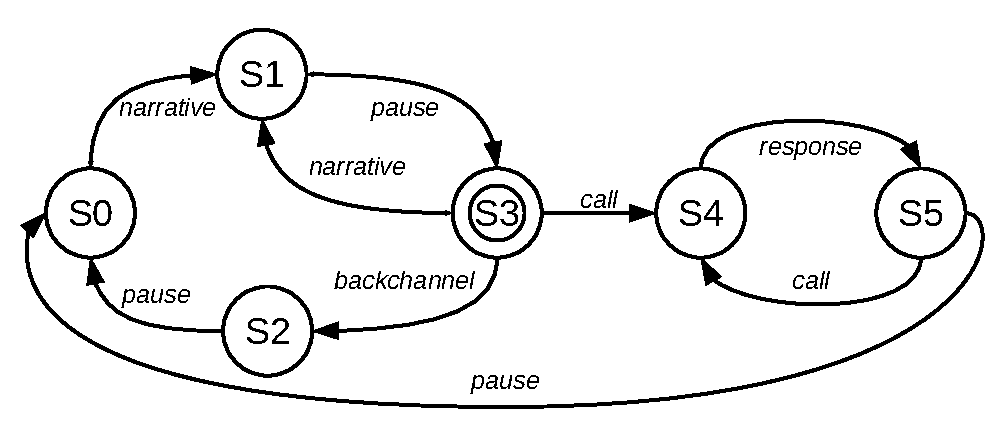
\includegraphics[width=0.65\textwidth]{gibbon_figure03.pdf}
\caption{\label{fig:fig03}Sketch of discourse grammar for interactive orature as an iterative transition network.}
\end{figure}

The cyclical linear grammar approach suits the Ega parable very well. In Figure\,\ref{fig:fig03} the iterative dialogue flow is represented in transition network format, showing inclusive cyclic patterning, i.e. a system with one cycle fully enclosed inside another (there are many other types but they do not apply in this context). The sequence of iterations can be formalised by means of a weakly equivalent right branching (or left branching) linear grammar.\footnote{Right-branching Type 3 grammar (‘|’ for options):
$\newline
\hspace*{30pt}S0 → narrator ~ S1 \newline
\hspace*{30pt}S1 → pause ~ S3 \newline
\hspace*{30pt}S2 → pause ~ S0 \newline
\hspace*{30pt}S3 → narrator S1~|~S3 → backchannel~S2~|~S3 → choir~S4 \newline
\hspace*{30pt}S4 → response ~ S5 \newline
\hspace*{30pt}S5 → choir ~ S4 ~ | ~ S5 → pause ~ S0$}
However, the transition network format of Figure\,\ref{fig:fig03} has greater heuristic visualisation value than grammar rule notation. An equivalent, though less perspicuous, regular expression can also be formulated.

The iterative linear grammar with inclusive cycles is realistic in real time and real memory space. It does not seem necessary to model the development of  dialogues like this as becoming ever more deeply embedded and requiring ever more nonlinear increases in time and memory space as the dialogue unfolds. The formal parallels between the dialogue model and cyclical prosodic models suggest that this dialogue grammar should be interpretable physically as a rhythm generating or accepting oscillator with inclusive cycles at multiple frequencies, which relates easily to cyclical linear models of prosody. This is to be demonstrated in the following sections on the phonetics of rhythm.

The including and included iterations have flexible assignments to locutions, especially in the \textit{narrator} turns and do not necessarily constitute a `strict layer hypothesis' \cite{selkirk1984}. Four inclusive cycles are defined by the FSA:
\vspace{-10pt}
\begin{enumerate} \itemsep -5pt
\item Local (included) cycles:
\vspace{-12pt}
	\begin{enumerate} \itemsep -5pt
	\item[] \textit{narrative-pause} cycle within a narrative turn;
	\item[] \textit{narrator-responder} cycle, with pauses, intervening within a narrative turn;
	\item[] chanted \textit{caller-choir} cycle, complementary to the \textit{narrator-responder} cycles;
	\end{enumerate}
\vspace{-5pt}
\item Global (including) cycle with restart of local cycles:
\vspace{-10pt}
	\begin{enumerate} \itemsep -5pt
	\item[] \textit{pause} return to \textit{narrative} start state.
	\end{enumerate}
\end{enumerate}
\vspace{-10pt}
Cycles, of the kinds shown in Figure\,\ref{fig:fig03} do not necessarily reflect a rhythmic pattern; the inverse is true, however: a rhythmic pattern is expressible as a cycle, given additional time and frequency constraints. The \textit{caller-choir} cycle in particular is a strong candidate for resonant oscillation with the coupling function of rhythm, as a chanted or sung context of \textit{caller-choir} pairs.

The task facing the following annotation-based phonetic analysis and acoustic phonetic signal processing is to investivate the empirical physical grounding for the different rhythms in the \textit{narrator-responder} and \textit{caller-choir} sequences.

%%%%%%%%%%%%%%%%%%%%%%%%%%%%%%%%%%%%%%%%%%%%%%%%%%%%%%%%%%%%%%%%%
%%%%%%%%%%%%%%%%%%%%%%%%%%%%%%%%%%%%%%%%%%%%%%%%%%%%%%%%%%%%%%%%%

\section{An inductive approach: rhythmic modulation}

\subsection{Phonetic preliminaries: annotation mining}

\begin{figure}[ht]
\centering
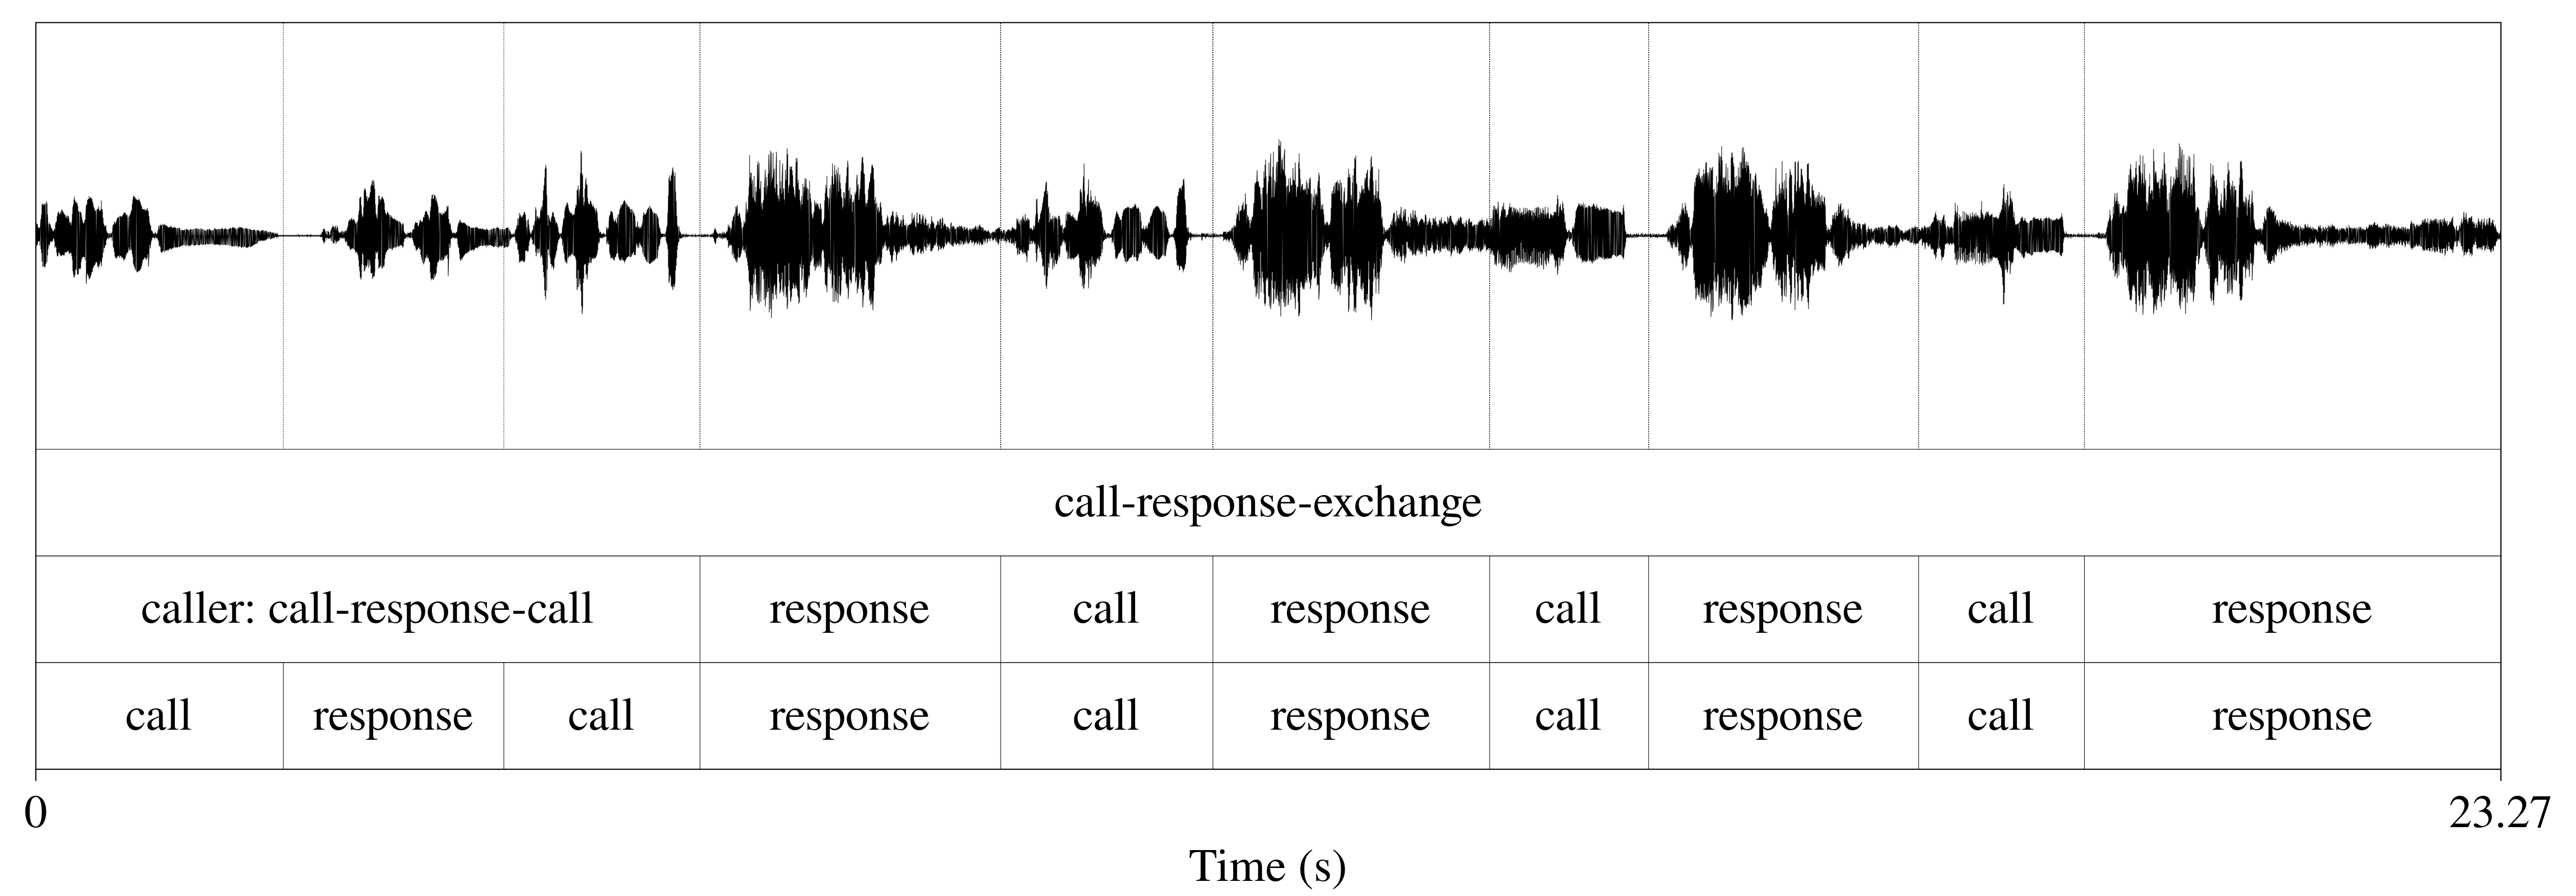
\includegraphics[width=0.98\textwidth]{gibbon_figure04.png}
\caption{\label{fig:fig04}Segment of Ega orature event annotation comprising \textit{caller-choir} iterations (posterised Praat screenshot).}
\end{figure}

A set of informal descriptive hypotheses are formulated:
\vspace{-10pt}
\begin{itemize} \itemsep -5pt
    \item[H0:] The presence of rhythmic beats cannot be identified in the speech signal.
    \item[H1:] The presence of rhythmic beats can be found by visual inspection of the waveform of the speech signal.
    \item[H2:] Rhythmic beats can be statistically described.
    \item[H3:] Rhythmic beats can be dynamically modelled in the time domain.
    \item[H4:] Rhythmic beats can be modelled in the frequency domain.
\end{itemize}
\vspace{-10pt}
H0 represents a sceptical view sometimes found in the literature. The hypotheses H1 to H3 represent goals for the time domain annotation-based analysis and are not incompatible but increasingly detailed. H4 represents the perspective of Rhythm Formant Analysis, to be addressed in the next section. The hypotheses are necessarily informal in view of the tiny data. H1 is immediately confirmed by inspection of Figure\,\ref{fig:fig04} and Figure\,\ref{fig:fig05} mid panel, and Table\,\ref{table:table01} provides simple evidence for H2. H3, H4 and H5 are argued for below (cf. Figure\,\ref{fig:fig05} and Figure\,\ref{fig:fig06}).
\begin{table}[ht]
\centering
\caption{Rhythm unit durations and periodicity of \textit{caller-choir} categories}
\vspace{0.2cm}
\label{table:table01}
\begin{tabular}{|l|c|c||c|c||c|c|}
\hline
\textbf{Item}	& \textbf{caller-d}	& \textbf{caller-p}	& \textbf{choir-d} & \textbf{choir-p} & \textbf{caller-choir-d} & \textbf{caller-choir-p}\\
\hline\hline
cr1:	& 2.337	& 0.428	& 2.08	& 0.481	& 4.417	& 0.226\\
\hline
cr2:	& 1.852	& 0.54	& 2.838	& 0.352	& 4.69	& 0.213\\
\hline
cr3:	& 2.004	& 0.499	& 2.612	& 0.381	& 4.616	& 0.217\\
\hline
cr4:	& 1.501	& 0.666	& 2.549	& 0.392	& 4.05	& 0.247\\
\hline
cr5:	& 1.565	& 0.639	& 3.931	& 0.254	& 5.496	& 0.182\\
\hline\hline
mean:	& 1.852	& 0.54	& 2.802	& 0.357	& 4.654	& 0.215\\
\hline
SD:	& 0.305	& 3.279	& 0.616	& 1.623	& 0.476	& \\
\hline
CoV:	& 0.165	& 6.061	& 0.22	& 4.545	& 0.1	& \\
\hline
\end{tabular}
\end{table}

The recording was annotated with participant turns, combining qualitative decisions on descriptive categories with time-stamped intervals in which these categories occur (see Figure \ref{fig:fig04} for a segment of the annotation). Results of the annotation and a basic descriptive analysis are shown in Table \ref{table:table01}. The low coefficients of variance for the sequences, together with the alternating durations between the \textit{narrator-responder} and \textit{caller-choir} turn exchanges, are simple time domain indications of long-term rhythmic properties.

\subsection{Modulation}

The abbreviations FM (frequency modulation) and AM (amplitude modulation) are familiar from radio broadcasting. In general, FM broadcasts use an HF carrier signal of around 100 MHz, modulated by lower frequency audio modulation up to 15kHz, and AM broadcasts use carrier frequencies below 30 MHz with more restricted audio modulation frequencies of 550 to 1720 Hz. The terms FM and AM can apply in any frequency range and are used here advisedly rather than `F0 estimation' in order to emphasise the general theoretical basis for the acoustic speech analysis and to underline the parallel AM and FM channel structure.

Modulation is the modification of a higher frequency carrier signal with a lower frequency information signal. The basic speech carrier signal is the fundamental frequency (F0) produced by phonation in the larynx, but whispering and obstruent noise are also carrier signals. The carrier signal is complex and in the case of F0 at the frequency $f$ also contains harmonics at integer multiples of $f$: $f, 2f, 3f, 4f, ...$.

The speech carrier signal is modulated directly at source in the larynx by lower frequency FM information signals (tone, pitch accent, intonation) and indirectly by AM air pressure variation (loudness) and oral-nasal filtering (consonants, vowels, certain voice quality features). The speech carrier frequency has an order of magnitude of $10^2$, between about 60~Hz and 500~Hz, depending on gender, age, emotionality and other factors. Low frequency modulations have much lower frequencies, with 50~Hz or less for consonants, around 10~Hz for vowels, 4~Hz for syllables, 1~Hz for words, 0.3~Hz for phrases, very approximately, depending on individual habits, speech rate, style, register and genre. Frequencies of the discourse rhythms of rhetorical structuring and turn-taking are considerably lower, about 0.1\,Hz to 0.01\,Hz.

FM and AM in speech have specific properties and also different roles in communication: noise, for example, is essentially amplitude modulation: frequency modulation is less sensitive to noise, explaining why, in teleglossia, communication at a distance, the speech rhythm and melody of a speaker, for example in the next room, can often be followed, but not the speaker's words, and why whistling, horns and melodic drums are used for teleglossic communication in many parts of the world.

\subsection{Rhythm Formant Theory (RFT): spectral patterning}

\begin{figure}[ht]
\vspace{-10pt}
\centering
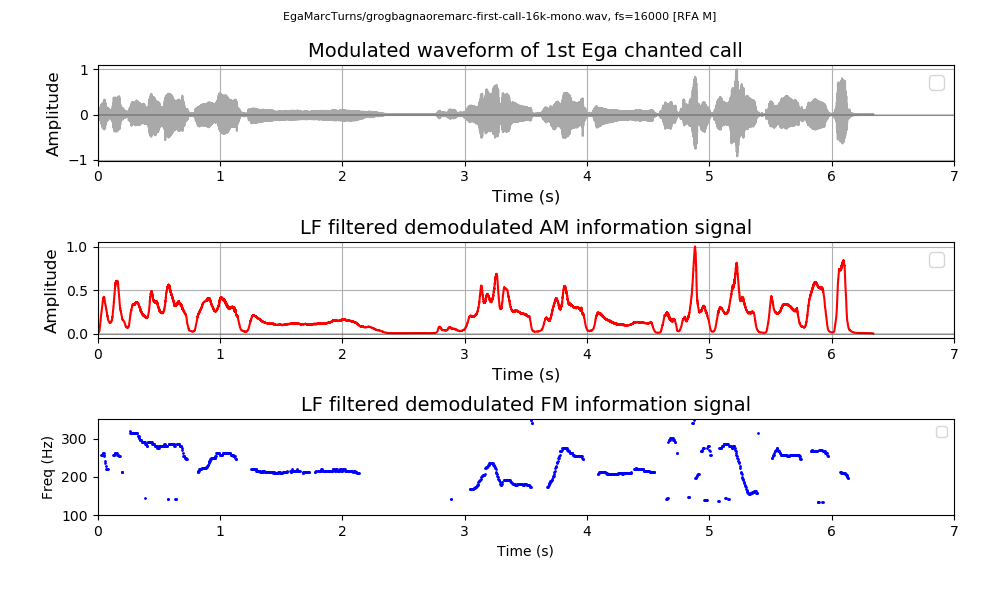
\includegraphics[trim={1.5cm 1.5cm 0 0}, clip, width=0.99\textwidth]{gibbon_figure05.png}
\vspace{-10pt}
\caption{\label{fig:fig05}Modulated waveform (upper panel), demodulated LF AM information signal (centre panel), demodulated LF FM information signal (lower panel).}
\vspace{-10pt}
\end{figure}

\begin{figure}[ht]
\centering
%\includegraphics[trim={1.5cm 1.5cm 0 0}, clip, width=0.95\textwidth]{GGMfirstnarration.png}
%\includegraphics[trim={1.5cm 1.5cm 0 0}, clip, width=0.95\textwidth]{GGMfirstcall.png}
{\footnotesize A. \textit{narrator-responder} exchanges following first \textit{caller-choir} exchanges (23\,s FFT window)}

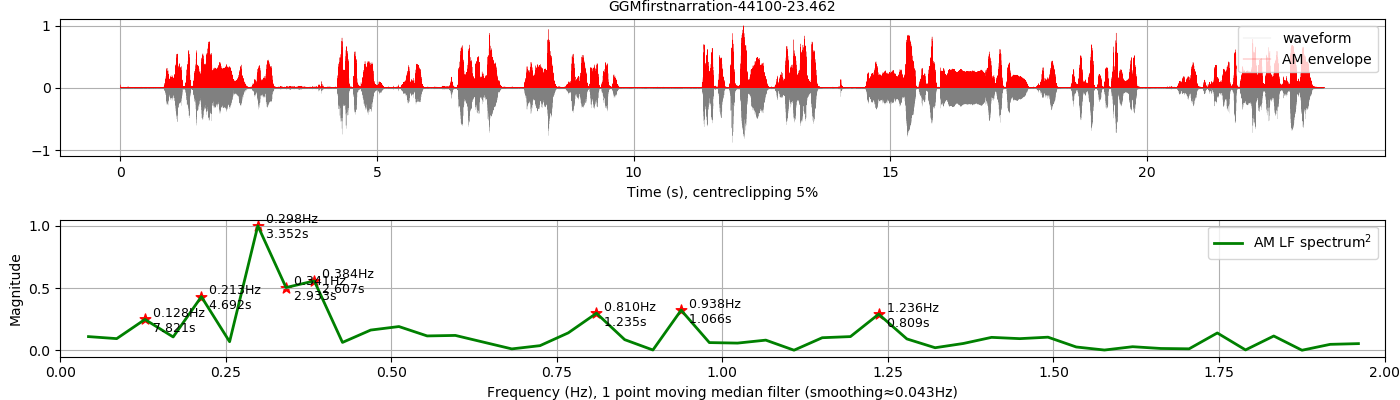
\includegraphics[width=0.99\textwidth]{gibbon_figure06A.png}

{\footnotesize B. First \textit{caller-choir} exchanges (23\,s FFT window)}

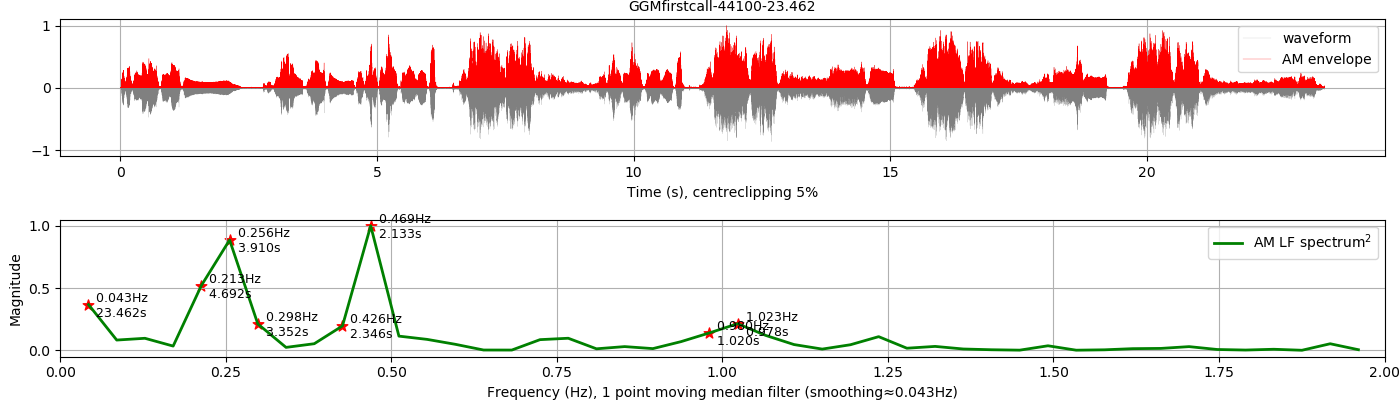
\includegraphics[width=0.99\textwidth]{gibbon_figure06B.png}

{\footnotesize C. Complete parable (300\,s FFT window)}

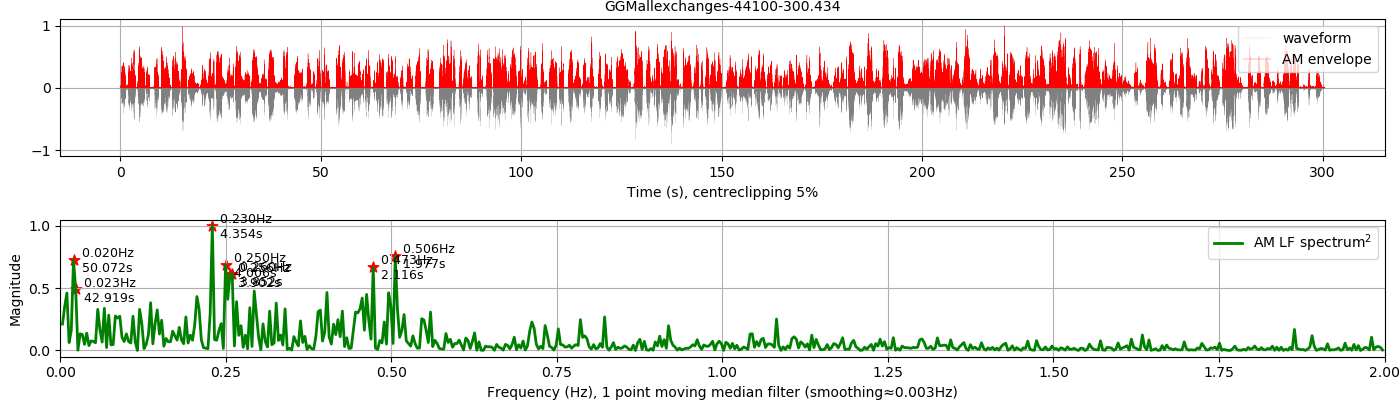
\includegraphics[width=0.99\textwidth]{gibbon_figure06C.png}
\caption{\label{fig:fig06}RFA: upper panels, waveform and amplitude envelope; lower panels, long-term spectrum of the selected event with conspicuous rhythm formants and smaller higher frequency formants.}
\end{figure}
\noindent
Rhythm Formant Theory is a further development of Speech Modulation Theory and addresses the task of the hearer (or the phonetician, or the automatic speech recognition application, in demodulating and then analysing the structure of the speech signal. The underlying idea in RFT \cite{gibbonsp2018, gibbonjipa2021, gibbonsp2022} is that speech rhythms are not only identifiable as intervals between beats or as beat rate per second in the time domain, but also, and in more detail, as low frequency spectral magnitude peaks, the rhythm formants. Over the entire spectral frequency range there are magnitude peaks at specific frequencies, in particular the peak frequencies of the LF AM and FM rhythm formants, the MF (medium frequency) carrier signal frequency (F0), and the HF peak frequencies of the harmonics of the carrier signal and of the HF phone formants as modulations of the harmonics.

The term \textit{formant} emphasises that, except for the different frequencies, the acoustic definition of LF rhythm formants as spectral peaks is the same as for the HF phone formants which constitute consonants and vowels, which are spectral peaks above and below 1\,kHz. The LF rhythm formants are spectral peaks above and below 1\,Hz, with frequencies between 0.3\,Hz and 10\,Hz (periods of 3\,s to 100\,ms) for the `linguistic rhythm' \cite{libermanprince1977} of syllables, words and phrases, and below approximately 0.3\,Hz (periods of $\rangle\rangle$3\,s or more, in the present analysis 300\,s) for rhetorical or discourse rhythms. Rhythm formants in both FM and AM LF spectra are relevant for rhythm analysis \cite{gibbonsp2018, gibbonjipa2021, gibbonsp2022, gibbon4urua2022}, but in the present contribution attention is restricted to the AM rhythm formants.

The Rhythm Formant Analysis (RFA) procedure associated with RFT processes the LF information-carrying speech signal, Figure\,\ref{fig:fig05} top panel, in 5 steps. First, the AM is demodulated, in the present analysis by taking the absolute values, i.e. full-wave rectification, of the signal. Second, the rectified signal is low-pass filtered at 10 Hz; the low-pass filtered rectified signal can be seen as a possible acoustic correlate of the phonological sonority curve, Figure\,\ref{fig:fig05} mid panel. Third, the low-pass filtered rectified signal is analysed by Fast Fourier Transformation (FFT). Fourth, the resulting low frequency spectrum is analysed for rhythm formants, i.e. high magnitude peaks in the spectrum and, fifth, the bandwidth of the formants determines the degree of rhythmicity or resonance at the formant frequency $f_{formant}$. Similarly, the FM envelope is demodulated any analysed, Figure\,\ref{fig:fig05} bottom panel.

The RFA procedure is applied to the \textit{caller-choir} iteration extract, shown in Figure\,\ref{fig:fig04} and the result is visualised in Figure\,\ref{fig:fig06}. The top panel of Figure\,\ref{fig:fig06} shows the waveform and the demodulated AM envelope in the time domain, as outlined in the previous section. The demodulated AM envelope is then transformed by applying the FFT in a window covering the whole \textit{caller-choir} sequence.

Panel A (top) of Figure\,\ref{fig:fig06} shows a single, relatively broad rhythmic range between 0.25\,Hz and 0.5\,Hz, which indicates \textit{narrator} turns of varying length. The smaller peaks anove 0.75\,Hz relate to shorter phrases, words and syllables of turns, and backchannel turns of the \textit{responder}, which are standardly `sese', roughly meaning ``Aha!'', though other particles of astonishment or disbelief occur.

It is also clear on visual inspection of panel B (centre) of Figure\,\ref{fig:fig06} that there are two main rhythm formants in the choral chanting, each with narrow bandwidth and thus high rhythmicity or resonance, neither of which covers the same spectral range as the narrative rhythm formant in panel A. The result for the \textit{caller} and \textit{choir} sequences is particularly interesting. Using the annotation time-stamps, it was predicted that a spectral frequency of 0.54\,Hz can be found for the \textit{caller} turns, 0.357\,Hz for the \textit{choir} turns and 0.215\,Hz for the combined \textit{caller-choir} exchanges, noting that there are outliers in each case. What is found is, in fact, rather close: in the centre panel of Figure\,\ref{fig:fig06} is a broader formant around 0.256\,Hz and a narrower formant around 0.469\,Hz. The first of these includes both the predicted 0.215\,Hz and 0.357\,Hz frequencies, with \textit{caller} and \textit{choir} merging into one formant region, while the second borders on 0.54\,Hz, for the combined \textit{caller-choir} exchanges. The result is approximate, and would need more detailed analysis, but tendentially the prediction H4 is borne out. That the procedure is generalisable to syllable-sized and word-sized rhythms has been shown elsewhere \cite{gibbonjipa2021}.

Moving on to panel C, the fragment just discussed is not the only such sequence in the story-telling event, and it is fair to predict that the same rhythm formants will be found in other \textit{caller-choir} occurrences in the parable. In fact, if these \textit{caller-choir} sequences are prominent enough, they will be visible in the low frequency spectrum for the entire event in spite of the wide range of other low frequency spectral frequencies, leading to a more specific hypothesis:

\vspace{-5pt}
\begin{itemize} \itemsep -5pt
    \item[H5:] The conspicuous rhythmic spectral properties of the first \textit{caller-choir} sequence are repeated in the later sequences, and are sufficiently prominent to be visible in a spectral analysis of the entire story-telling event.
\end{itemize}

The result of the holistic low frequency spectral analysis is shown in panel C (bottom) of Figure\,\ref{fig:fig06}. The predicted frequencies are still plainly in evidence in the spectrum of the entire utterance, and, informally, H5 is supported. The spectrum is more ragged, noisier, (or more precisely: more detailed), because of some frequency variation between the different \textit{caller-choir} exchanges, because of the presence of other frequencies from the \textit{narrator-responder} exchanges and because of the much higher spectral resolution resulting from use of a longer FFT time window of nearly 5 minutes.

Taking up the concepts introduced in the discussion of discourse functionality in linguistic stylistics, it is suggested that the regular low frequency rhythms which are detectable in the spectrum are major coupling forms in orature, specifically in the \textit{caller-choir} exchangef sequences, with several coupling functions: first, to identify the \textit{caller-choir} type of dialogue act; second, to bind the two parts of the dialogue act syntagmatically; third to identify instances of coherent sequences of \textit{caller-choir} pairs. This perspective is motivated by previous work on other long-term spoken events such as news-reading, story-reading and poetry recitation \cite{gibbonjipa2021, gibbonsp2022, gibbon4urua2022}.

\subsection{Combining frequency and time domains: the LF spectrogram}

\begin{figure}[ht]
\centering
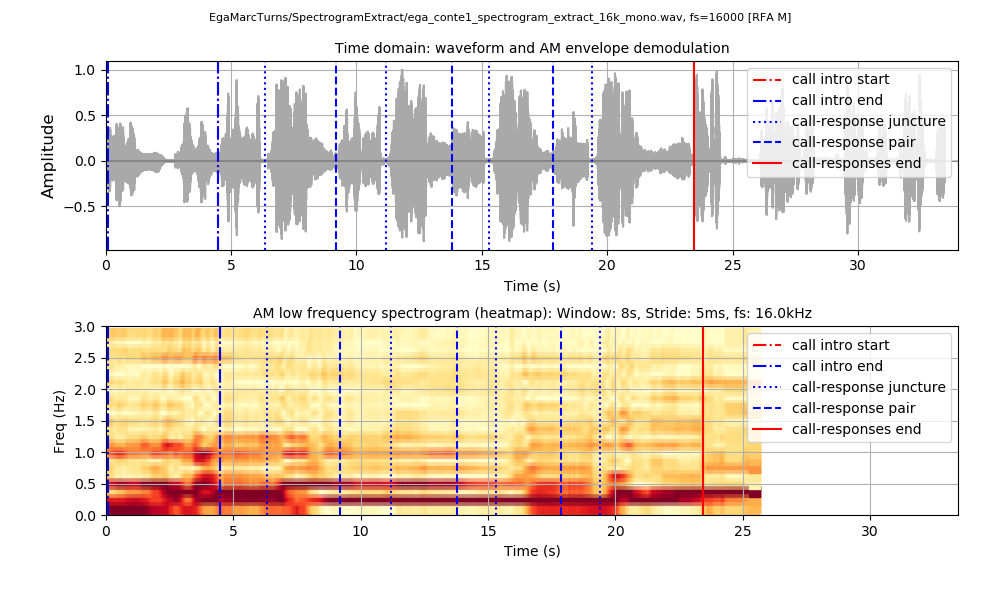
\includegraphics[trim={1.5cm 1cm 0 0}, clip, width=0.95\textwidth]{gibbon_figure07.png}
\caption{\label{fig:fig07}Low frequency spectrogram of the first \textit{caller-choir} sequence of the Ega parable (empty trailing context due to stride length; slight misalignment due to stride rounding).}
\end{figure}
\begin{figure}[ht]
\centering
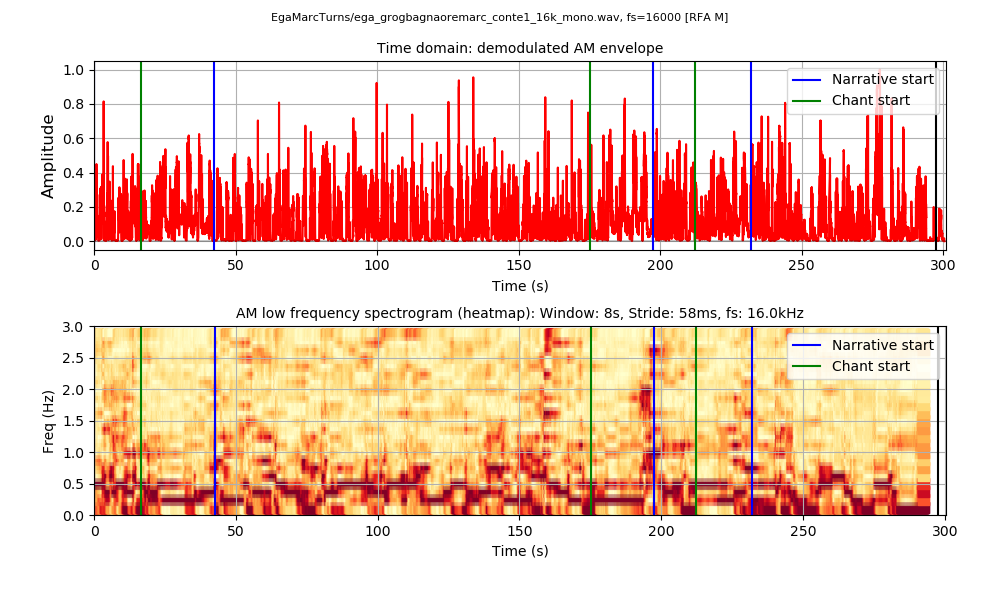
\includegraphics[trim={1.5cm 1cm 0 0}, clip, width=0.95\textwidth]{gibbon_figure08.png}
\caption{\label{fig:fig08}Long-term LF spectrogram of the entire Ega parable; window size 8 s, strides 0.75\,s, with episode (narrator and chant turn) boundaries.}
\end{figure}


\begin{table}[ht]
\centering
\caption{Annotation of the complete parable with narrative and chant episodes}
\vspace{0.2cm}
\label{table:table02}
\begin{tabular}{|l||l||c|c||c|}
\hline
\textbf{Tier} & \textbf{Label} & \textbf{Start} & \textbf{End} & \textbf{Duration}\\
\hline\hline
Episodes	&	\_	&	0.000	&	0.146	&	0.146\\
Episodes	&	Narrative	&	0.146	&	16.684	&	16.538\\
Episodes	&	Chant	&	16.684	&	42.463	&	25.779\\
Episodes	&	Narrative	&	42.463	&	175.125	&	132.662\\
Episodes	&	Chant	&	175.125	&	197.426	&	22.301\\
Episodes	&	Narrative	&	197.426	&	212.238	&	14.812\\
Episodes	&	Chant	&	212.238	&	231.901	&	19.663\\
Episodes	&	Narrative	&	231.901	&	297.499	&	65.598\\
Episodes	&	\_	&	297.499	&	300.434	&	2.935\\
\hline
\end{tabular}
\end{table}
\noindent
The information provided by the long-term LF spectrum is solely in the frequency domain, a generalisation over the whole temporal extent of the story-telling. The spectrum provides no information about possible variation of rhythm formants in time. For additional temporal information, a long-term LF spectrogram containing a sequence of many shorter spectral slices is needed, in which all of the \textit{narrator-responder} and \textit{caller-choir} exchanges can be placed. Figure\,\ref{fig:fig07} shows an annotated segment, which includes 8\,s of following context for the \textit{caller-choir} exchange, required by the 8\,s long FFT window required by the low frequency analysis, and the low frequency spectrogram for the segment.

The sampling frequency of 16\,kHz and the spectrogram spectral slice window of 8\,s provide adequate frequency resolution for the expected frequencies at around 0.2\,Hz (period 5\,s) and 0.4\,Hz (period 2.5\,s). However, the 8\,s FFT window comes at a cost, namely very low temporal resolution. This low temporal resolution is compensated by extremely short window strides of only 5\,ms. The long FFT window requires the inclusion of at least 8\,s of following context in order to capture the whole final signal segment, leaving a blank space in the spectrogram after the last full 8\,s window, corresponding to the duration of the FFT window. The final spectral slice appears at the beginning of the blank interval. However, the massively overlapping stride interval of 5\,ms, which is extremely short in relation to the duration of the 8\,s spectral slice window, recoups the lost time resolution. The very slight misalignment of the spectrogram bars and the waveform bars in the visualisation is due to uncorrected decimal rounding of the stride duration, but is not important for the present purpose.

The vertical boundary bars in Figure\,\ref{fig:fig07} mark the boundaries of exchange types, and are derived from the annotation shown in Figure\,\ref{fig:fig04}. In the spectrogram the two expected rhythm formants at around 0.2\,Hz and 0.5\,Hz are clearly visible in the central section as two distinct narrow bandwidth horizontal bars, which merge into a broader bandwidth horizontal bar in the final section, and correspond to the rhythm formants shown in Figure\,\ref{fig:fig06}, panel B. The \textit{caller} turns are shorter than the \textit{choir} turns and the first and fourth \textit{caller} turns do not share this degree of rhythmicity or resonance with the choir. The third \textit{choir} turn is also somewhat irregular.

The positions of the two \textit{caller-choir} rhythm formants in the timeline are very clear, in contrast to the \textit{narrator-responder} formant. The two rhythm formants are in a quasi-harmonic octave relationship to each other, one being twice the frequency of the other, due to the binary structure of the \textit{caller-choir} grouping. The quasi-harmonic two-formant pattern can be interpreted as a linearly organised prosodic hierarchy, represented by cycles in the oscillator automaton in Figure\,\ref{fig:fig03}, along the lines of coupled oscillator theory.

So far, the spectrogram of just one \textit{caller-choir} sequence was discussed. A more ambitious validity check is on whether the pattern is repeated in the two following similar \textit{caller-choir} sequences, in which varying \textit{caller} content occurs, but with the same \textit{choir}. The low frequency spectrogram for the entire parable is shown in Figure\,\ref{fig:fig08}, with narrative and chant episodes marked. The time window for each spectral slice is again 8\,s, with the same number of equally spaced strides, but here each stride is 58\,ms in duration, due to the 5\,min FFT window. Figure\,\ref{fig:fig08} starts with the \textit{narrator-responder} cycle, followed by the \textit{caller-choir} chant cycle, \textit{narrator-responder} cycle, \textit{caller-choir} chant cycle, \textit{narrator-responder} cycle, \textit{caller-choir} chant cycle, \textit{narrator-responder} cycle, closing with the moral and the narrator's name. The boundary time-stamps are given in Table\,\ref{table:table02} in order to facilitate checking with Figure\,\ref{fig:fig08}.

In summary, the expected dual rhythm formant bars for the three \textit{caller-choir} exchanges are present, at about 30\,s, 180\,s and 220\,s, and provide further informal support the hypotheses H2, H3, H4 and H5. The intervening \textit{narrator-responder} alternations are complementary to the \textit{caller-choir} cycles, and can be seen to have their own entirely different shorter-term timing properties. It is beyond the scope of the present study to investigate other details. It is sufficient for the present study to point out that there are in fact clear spectral differences in segments of the discourse, that they evidently relate to different kinds of turn in the interaction, and that pessimism about identifying rhythm in the physical signal, at least in its discourse functions, is not justified.

\section{Summary and conclusion}

This contribution explores functional, structural and physical properties of speech rhythms in the interactive narration of a parable in the endangered Ega language, south central Ivory Coast, recorded during a fieldwork project, a small and rare example of traditional orature. The village orator has two roles, as \textit{narrator} of the parable with feedback from his designated \textit{responder}, and as \textit{caller} in chanted interaction with a responding audience as \textit{choir}.  The methodology is an interdisciplinary combination of qualitative and quantitative analyses. Relevant functions of speech rhythm are characterised as coupling, a concept from linguistic stylistics, and iterations of matching functional and structural cohesion in the temporal rhythm domain are described with a cyclical linear model. Annotation analysis provides a hybrid qualitative-quantitative bridge to acoustic phonetic signal analysis, and finally spectral peaks which distinguish between different turn and exchange types are interpreted as rhythm formants with a high level of rhythmicity or resonance. The signal processing procedure is based on \textit{Rhythm Formant Theory} and its associated \textit{Rhythm Formant Analysis} methodology and provides physical grounding for rhythm theories, embedded in a background of poetic culture.

In conclusion, it was shown that functional, structural and causal physical accounts can combine to explain the overall picture of how speech rhythms work in interactive orature: \textit{discourse rhythms} have a \textit{coupling} function for the accompanying locutions, are given hermeneutic motivation by functional analysis, and are structured by means of an \textit{iterative linear oscillator} (in the formal grammar sense of `linear'), and realised with \textit{causal physical grounding} as \textit{rhythm formants} with specific frequency, amplitude and bandwidth properties.

Further applications in discourse analysis and in other disciplines such as automatic spoken language analysis, recognition and identification, as well as in spoken language system evaluation and L2 fluency assessment are anticipated. Not all rhythms, whether in syllable, word, and phrase time domains or in the long time domains of discourse turns, can be detected all of the time. But it helps to look in the right places.

\section{Acknowledgments}
%\addcontentsline{toc}{section}{Acknowledgments}

Warmest thanks are due to co-PI Firmin Ahoua and our initial Ega contact, Père Oku Towe Cyprien, for initiating the Ega fieldwork project. For annotation and archiving the video data I am indebted to Sophie Salffner as fieldwork partner in Côte d'Ivoire. Above all, my gratitude goes to the experienced village orator, the late Gnaoré Grogba Marc, \textit{chef de village} of Gnieguédougou, Côte d'Ivoire, to Paul, his responder, and to the Ega community, for their warm welcome and their willingness to proudly demonstrate their complex orature tradition. Not least, acknowledgement is due to the inspiring pioneering fieldwork of Daniel Everett in realistically accounting for patterns in spoken dialogue and to Sascha Griffiths for many years of discussion on fieldwork and on the realistic description of spoken languages.


\printbibliography

\end{document}
